% SLOT MAPPING. The authoritative main.tex names this slot "04_opportunities".
% The content is the system-design section (formerly paper/04_system.tex). The
% authoritative filename is kept so the governing \input list is unchanged;
% only the file's contents differ from what the name suggests. The evaluation
% that followed it has no slot in the authoritative list and lives in
% sections/04b_evaluation.tex, pulled in by an ADDED \input line in main.tex.
% Source: sc-workshop-paper/paper/04_system.tex (prose unchanged).

\section{Design of \sysname}

\subsection{System Overview}

\sysname{} manages a single host-memory budget shared by two kinds of
resource: the language models backing an agent's reasoning and tool-calling
steps, and the scientific data artifacts those tools consume. The retention
arbitrator is the primary component and acts wherever memory pressure forces a
choice; the opportunistic prefetcher is deliberately subordinate to it. Both
score candidates with one value function, so a decision to stage and a
decision to keep are directly comparable rather than governed by separate
policies competing for the same memory.

\subsection{Residency States}

A resource sits in one of three states. \emph{Active} is serving---a model
answering requests on a device, an artifact activated in a live worker.
\emph{Released} is the opposite: the process is gone and the next use pays
full construction. Between them is \emph{held}, the state the arbitrator
budgets, in which the resource is not serving but the expensive part of making
it usable has been paid and is being kept. For a model that is parked weights
with the serving process, device context and allocator still alive, so
returning to active is a wake rather than a boot---782~s becomes 2.1~s. For an
artifact it is a resident worker holding the parsed structure across
invocations.

Held is the only state that costs host memory, and its two forms are the same
object to the operating system: anonymous memory in a live process, invisible
to any file-backed cache and charged to one allocation. Hence one arbitrator
for both---a parked model and a retained database compete for exactly the same
bytes.

\subsection{The Retention Arbitrator}

At each decision point the arbitrator selects the set of resources to leave in
the held state. Let $g(r)$ be the memory $r$ occupies while held, $B$ the
budget, and $\Delta t(r)$ the estimated time until $r$ is next required.
Writing $\mathrm{cold}(r)$ for the cost of producing $r$ from scratch and
$\mathrm{ready}(r)$ for the cost of resuming it from the held state, the
saving retention buys is $\mathrm{cold}(r) - \mathrm{ready}(r)$.

Neither obvious ranking of that saving works on its own. Ranking on the saving
itself is indifferent to when the resource is next needed, so one required in
ten seconds and one required in three hours compete equally and the budget
fills with what will not be used soon. Ranking on saving per unit of
time-to-use collapses the difference between a large saving and a small one
whenever both are imminent. Each is correct in exactly the regime where the
other fails, so \sysname{} applies them conditionally, on either side of an
explicit planning horizon $H$:

\begin{equation}
v(r) \;=\; \bigl(\mathrm{cold}(r) - \mathrm{ready}(r)\bigr)
           \cdot \frac{H}{\max\!\left(\Delta t(r),\, H\right)}
\label{eq:value}
\end{equation}

\noindent ranking by \emph{value density} $v(r)/g(r)$---seconds of stall
avoided per gigabyte held. Inside $H$ the discount is~1 and candidates are
compared on absolute seconds saved, so a small imminent resource cannot
outrank a large one merely by being sooner; outside it value decays as
$H/\Delta t$, so a resource that will not be touched for a long time surrenders
its memory to one that will.

$H$ is a tunable, and the natural setting is on the order of the workflow's
typical inter-step gap. It is also what lets staging and retention be scored
in one currency (Section~\ref{sec:prefetch}).

Device memory is a separate, smaller capacity, so only a model displaced from
it becomes a candidate for the held state. The arbitrator decides in the same
step whether that candidate is worth its host memory or should be released
outright.

\subsubsection{Selection Under Indivisibility}


Held resources cannot be partially surrendered. Half a model's weights serve
no requests, and a partially retained structure does not answer queries, so
release is all-or-nothing. Selection is therefore a subset choice under a
capacity constraint rather than a sequence of independent evictions, and
\sysname{} evaluates it as one: it searches for the highest-value set that fits,
rather than repeatedly discarding the worst-ranked resident. The distinction
matters whenever admitting one large resource requires releasing two smaller
ones---a decision single-victim eviction cannot express. Ties are broken
toward the smaller total footprint, so equal value never costs extra budget.


\subsubsection{Horizon Estimation}
\label{sec:horizon}

The arbitrator's only external input is $\Delta t(r)$, and \sysname{} obtains
it by combining the two signals characterised in Section~\ref{sec:insights}: a
planner's declared step sequence, which reaches far ahead but locates poorly,
and a transition model over observed executions, which locates well but only
locally. The second covers exactly the region where the first is silent or has
been departed from.

The two merge into one predicted step sequence---the plan supplying structure,
the transition model correcting it near the present---in which each step
carries an expected duration. $\Delta t(r)$ is the summed duration between now
and the earliest predicted step requiring $r$. Each estimate also carries a
confidence, from the sources' agreement and the sharpness of the successor
distribution, which the arbitrator applies as a weight: an uncertain horizon
perturbs a ranking rather than forcing a decision.

One property of this estimator is load-bearing for the arbitrator. Lookahead
is bounded, so the predictor reports \emph{not required within $H$} rather
than \emph{not required again}. The arbitrator treats the two very
differently: the first is a low rank that still competes for spare memory,
while the second would be licence to discard. Preserving that distinction
keeps a resource eligible whenever the budget has room for it, independently
of how far ahead the estimate can see.

\subsection{The Opportunistic Prefetcher}
\label{sec:prefetch}

% EVALUATION FLOATS, DECLARED EARLY AND DELIBERATELY OUT OF SECTION.
% These belong to the evaluation and are cited there. They are
% declared here because a float cannot move backwards, and the evaluation
% opens partway down a page whose top is already committed by then --
% which is why that page previously carried no figure at all. Declared in
% this section's text, they can take that page's top slots. Per author
% preference, a reader flipping back one page beats figures piling up
% pages later.
%
% ORDER MATTERS HERE. fig:budget-sweep and fig:ablation are both figure*,
% and consecutive double-column floats stack into a slab with the
% single-column ones pushed beneath. Declaring the full-width budget sweep
% BEFORE the single-column stall ladder puts a one-column float between the
% two figure*s and breaks the stack. The evaluation's subsections are
% ordered to match, so citation order still runs forward.
\begin{figure*}[t]
\centering
% PLOT SPEC (kept for provenance; rendered by
% scripts/figures/make_figures.py -> figure_drafts/fig-budget-sweep.pdf)
%   MERGED FIGURE. The original spec put binding on a twin right-hand axis;
%   that violates the no-dual-axis rule, so binding became a separate float
%   (fig:topology-budget) and then, here, the lower ROW of this one. Both read
%   the same rows of results_tables/02_budget_sweep.md.
%   Top row: reduction vs \textsc{Never} for \textsc{Lru} and \sysname, one
%   column per device-slot count. Bottom row: binding \%, same columns,
%   shared x. Shaded span = where binding is 0. Packing thresholds at 283,
%   445 and 562~GB as vertical rules.
%
%   TODO (author): the zero-binding margin is a PREFETCH claim arriving from
%   a direction that flatters it. Per the project reporting rule, confirm the
%   binding==0 cells against the oracle-vs-LRU gap at the same budget before
%   this becomes a headline.
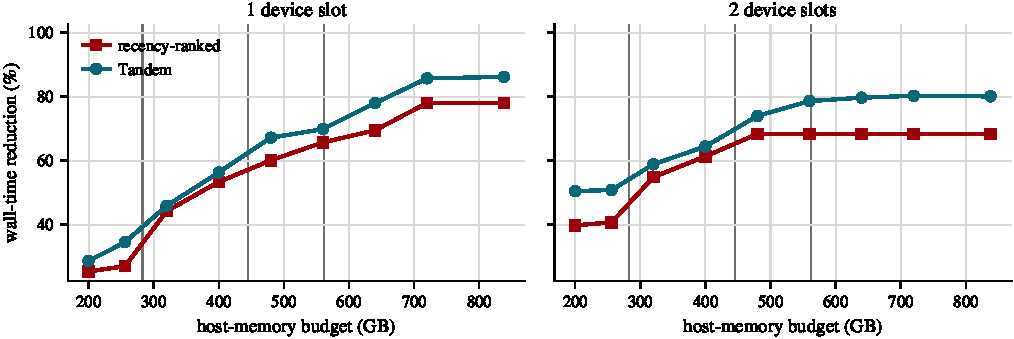
\includegraphics[width=0.95\textwidth]{figures/fig-budget-sweep}
\caption{Wall-time reduction against \textsc{Never} (top) and the share of
decisions in which memory pressure forced an eviction (bottom), by budget and
device capacity. Shading marks the span where no eviction ever occurs: the
policies separate most widely inside it, because with the arbitrator idle the
remaining margin is staging.}
\label{fig:budget-sweep}
\end{figure*}
\begin{figure}[tb]
\centering
% PLOT SPEC (kept for provenance; rendered by
% scripts/figures/make_figures.py -> figure_drafts/fig-stall-ladder.pdf)
%   grouped bars, stall seconds per arm (\textsc{Never}, \textsc{Lru}, 
%   \sysname) at 256~GB/1 slot and 560~GB/2 slots. Annotate each \sysname{} 
%   bar with its reduction over \textsc{Lru}.
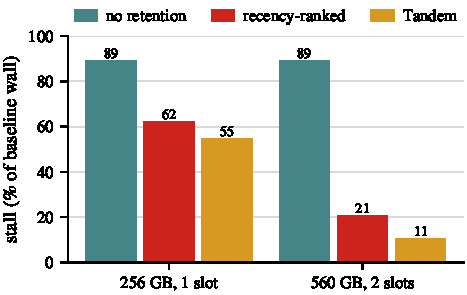
\includegraphics[width=\columnwidth]{figures/fig-stall-ladder}
\caption{Stall attributable to resource residency, by policy and
configuration.}
\label{fig:stall-ladder}
\end{figure}

The arbitrator acts on resources the workflow has already used. The prefetcher
acts on resources it has not: drawing on the same horizon estimates
(Section~\ref{sec:horizon}), it moves a resource toward residency before the
need arrives, so that construction or transfer overlaps computation rather
than blocking it.

Staging is scored in the same currency as retention, with one difference in
how the saving is computed. Retention saves the full $\mathrm{cold}(r) -
\mathrm{ready}(r)$ whenever the resource is next used, because the work is
already done. Staging saves only as much of that cost as fits in the interval
before the need---a stage that gets halfway leaves the remainder exposed. Its
benefit is therefore capped by $\Delta t(r)$, and Eq.~\ref{eq:value} applies
to that capped quantity.

\subsubsection{Slack First}

The prefetcher's default is to consume only \emph{slack}: memory the
arbitrator has left unclaimed. If a resource does not fit in unused budget the
stage is abandoned rather than funded by displacing something resident. That
restriction is what makes speculation safe here---a stage drawing only on
slack has its downside bounded by wasted bandwidth, since it cannot cost a
retention worth more, so its expected value stays positive across a wide range
of horizon quality instead of requiring precision to break even.

\subsubsection{The Outbid Path}


Restricting staging to slack forgoes the cases where a stage genuinely is
worth more than an incumbent, so \sysname{} permits displacement under four
conjunctive conditions. The stage's value density must exceed the incumbent's
by a margin wider than estimation noise, so that noise alone cannot reorder
them. The predicted window must be long enough to complete the stage, since a
partial stage trades a certain retention for a speculative saving. The
incumbent's own horizon must lie beyond $H$, placing it outside the window in
which candidates are compared on absolute savings. And the horizon estimate
must clear a confidence threshold, because displacement is the one staging
action whose cost slack does not bound. The conjunction is deliberately
conservative: the prefetcher is a slack consumer under normal conditions, and
the arbitrator, not speculation, stays in control of the budget.
